\documentclass[../DoAn.tex]{subfiles}
\begin{document}

Trong chương này, em sẽ trình bày chi tiết các công nghệ đã sử dụng trong quá trình xây dựng và phát triển hệ thống.

\section{Flutter}
\label{section:3.1}

Flutter là UI Framework có mã nguồn mở hoàn toàn miễn phí được phát triển và phát hành bởi Google giữa năm 2017. Đặc biệt, Flutter cho phép người dùng xây dựng các ứng dụng đa nền tảng từ cùng một codebase. Với Flutter, người dùng sử dụng một ngôn ngữ lập trình duy nhất - Dart cùng với codebase để tạo ứng dụng trên nhiều nền tảng như Android, iOS, Web, ... Ngôn ngữ Dart là ngôn ngữ có khuynh hướng thuần hướng đối tượng được Google phát triển và công bố năm 2011 với mục đích cung cấp ngôn ngữ hiện đại hơn, tối ưu cho client hơn và đặc biệt hỗ trợ đa nền tảng. Từ đó, em đã lựa chọn Flutter để xây dựng ứng dụng vì những ưu điểm nổi bật sau đây:

\begin{itemize}
    \item Phát triển ứng dụng nhanh.
    \item Chỉ cần viết một lần trong một mã nguồn có thể chạy cho tất cả các ứng dụng.
    \item Giao diện người dùng đẹp và linh hoạt.
    \item Hỗ trợ nhiều thành phần khác nhau và dễ chỉnh sửa.
    \item Ngôn ngữ kiểu tĩnh nhưng cú pháp hiện đại (tương tự Javascript, Java, Python).
    \item Có chứng năng hot reload, hot restart hỗ trợ nhanh trong việc lập trình, không phải chạy lại ứng dụng nhiều lần gây mất thời gian.
\end{itemize}

\section{Javascript}
\label{section:3.2}

Javascript viết tắt là JS. Javascript là một ngôn ngữ lập trình kịch bản dựa vào đối tượng phát triển, được sử dụng rộng rãi trong các ứng dụng Website và hỗ trợ hầu như trên tất cả các trình duyệt trên máy tính lẫn điện thoại.

Nhiệm vụ của Javascript là xử lý những đối tượng HTML trên trình duyệt, có thể can thiệp với các hành động như thêm/sửa/xoá các thuộc tính CSS và các thẻ HTML một cách dễ dàng. Có thể nói, JS chịu trách nhiệm chính trong việc tương tác với người dùng. Trong những năm gần đây, các nhà sáng lập đã đưa ra nhiều framework như NodeJS - chuyên dùng cho backend, ExpressJS\cite{ExpressJS} - là NodeJS framework và nhiều thư viện frontend khác như Angular, jQuery, ReactJS.

Việc ĐATN của em lựa chọn Javascript làm ngôn ngữ để xây dựng backend đảm bảo được phía server được hoạt động hiệu quả, nhanh gọn, hoàn thiện cao và bảo trì tốt.

\section{Platform NodeJs và Framework Express}
\label{section:3.3}

NodeJS là một nền tảng được xây dựng trên V8 Javascript engine\cite{V8_Javascript_engine} được viết bằng C++ và Javascript, nền tảng này được phát triển bởi Ryan Lienhart Dahl vào năm 2009. NodeJS ra đời cho phép các nhà phát triển của Javascript có thể chạy trên máy của mình dưới dạng ứng dụng độc lập. NodeJS sử dụng kiến trúc hướng sự kiện event-driven, mô hình non-blocking I/O làm cho nó nhẹ và hiệu quả hơn. Công đồng sử dụng Nodejs rất lớn mạnh, bên cạnh đó có rất nhiều website lớn đang sử dụng NodeJS để viết chương trình như: Ebay, Trello, Paypal, ...

Express là một framework mã nguồn mở miễn phí cho NodeJS. Sử dụng Express cho phép lập trình viên tạo dự bộ khung ứng dụng một cách nhanh chóng và đơn giản. Những lợi ích mà Express mang lại:
\begin{itemize}
    \item Xây dựng phần mềm trung gian có quyền truy cập vào cơ sở dữ liệu.
    \item Phát triển máy chủ nhanh chóng.
    \item Dễ gỡ lỗi khi viết mã nguồn.
    \item Hệ thống thư viện đa dạng, được phát triển và hỗ trợ nhiều bởi cộng động lớn.
\end{itemize}

Với những lợi ích đó, em lựa chọn NodeJS cùng Express để xây dựng máy chủ kết nối với ứng dụng real-time có thời gian trễ thấp, tiết kiệm được thời gian xây dựng hệ thống và giúp hệ thống dễ dàng chỉnh sửa và mở rộng.

\section{Socket.IO}
\label{section:3.4}

Socket.IO là một module trong NodeJS được nhà sáng chế tạo ra và phát triển từ năm 2010. Mục đích lớn nhất của Socket.IO là để tạo môi trường giao tiếp thuận lợi trên Internet giúp trả về các giá trị thực tại ngay thời điểm giao tiếp giữa các bên với nhau (thường là giữa server và client).

Các lập trình viên luôn ưu tiên Socket.IO ở vị trí số một bởi nó mang nhiều tính năng nổi bật như:
\begin{itemize}
    \item Bảo mật cao.
    \item Kết nối tự động với Server.
    \item Mã hoá nhị phân.
    \item Cho phép tạo kênh và phòng.
\end{itemize}

Vì hệ thống điều khiển xe Arduino cần có kết nối liên tục và có những phải hồi liên tục giữa ứng dụng với xe nên Socket.IO là một lựa chọn tốt, miễn phí và đem lại trải nghiệm tốt cho người dùng sử dụng hệ thống.

\section{Module NodeMCU Esp32}
\label{section:3.5}

ESP32 là một chip được tích hợp công nghệ Wifi và Bluetooth\cite{Bluetooth} với công nghệ tiêu thụ năng lượng cực thấp. Nó cung cấp một nền tảng tích hợp mạnh mẽ, đáp ứng nhu cầu hiệu năng tốt nhất, tính linh hoạt, thiết kế nhỏ gọn, hiệu suất cao và độ tin cậy trong nhiều ứng dụng. Các dòng chip ESP32 bao gồm ESP32-D0WDQ6, ESP32-D0WD, ESP32-D2WD và ESP32-S0WD.

Expressif đã thiết kế và sản xuất ra một số module để người dùng dễ dàng tiếp cận hơn với dòng chip ESP32. Các thành phần chính trên những module này bao gồm chip ESP32, bộ tạo dao động thạch anh, mạch ăngten, chỉ khác nhau về một số chức năng tuỳ từng phiên bản như số lượng chân GPIO, các thiết bị ngoại vi được thêm vào như: màn hình LCD, bảng cảm ứng, khe cắm thẻ SD, module máy ảnh, ... 

Phiên bản ESP32-WROOM-32 là một module vi điều khiển (MCU) Wifi (Wifi Fidelity) - BT (Bluetooth) - BTE (Bluetooth Low Energy) phổ biến và mạnh mẽ phục vụ cho nhiều ứng dụng khác nhau từ những ứng dụng đơn giản như điều khiển thiết bị, đọc giá trị cảm biến đến những nhiệm vụ phức tạp như mã hoá giọng nói, phát nhạc trực tuyến, ...

\begin{figure}[H]
    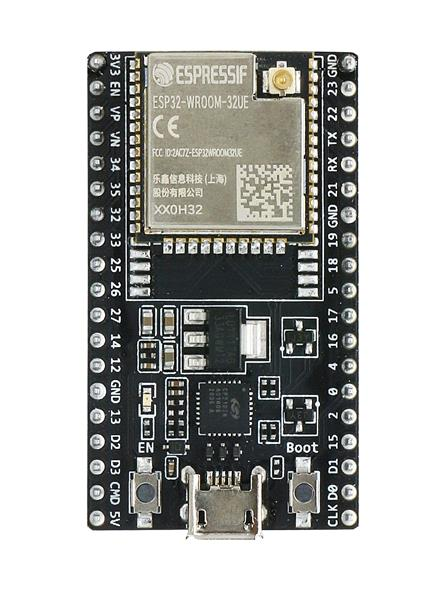
\includegraphics[scale = 0.6]{Hinhve/ESP32.jpg}
    \centering
    \caption{Module NodeMCU Esp32}
\end{figure}

Module này được xây dựng với lõi nhân là chip ESP32-D0WDQ6, chip được thiết kế để có thể mở rộng. Có 2 lõi CPU (Central Processing Unit) có thể kiểm soát riêng biệt và tần số xung đồ hồ dao động từ 80MHz đến 240MHz.

Một số ứng dụng của ESP32, đa số các ứng dụng của ESP32 được phục vụ cho các dự án IoT như:
\begin{itemize}
    \item Nhà thông minh.
    \item Robot công nghiệp.
    \item Nhận dạng giọng nói.
    \item Nhận dạng hình ảnh.
    \item Ứng dụng chăm sóc sức khoẻ.
\end{itemize}

Dưới đây là thông số kỹ thuật cơ bản của module ESP32-WROOM-32

\begin{figure}[H]
    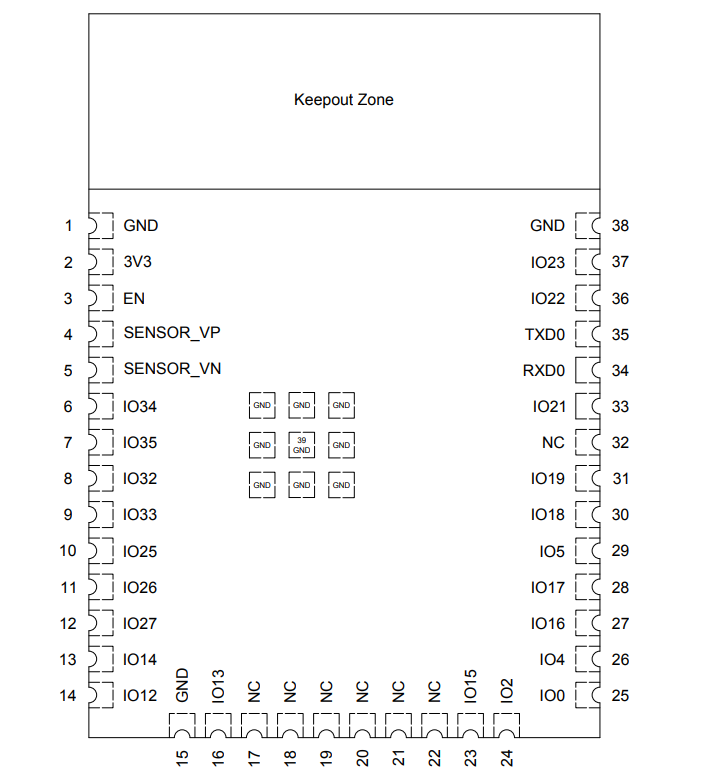
\includegraphics[scale = 0.6]{Hinhve/ESP32-Pin-Layout.png}
    \centering
    \caption{Sơ đồ bố trí chân của module ESP32-WROOM-32}
\end{figure}

\begin{figure}[H]
    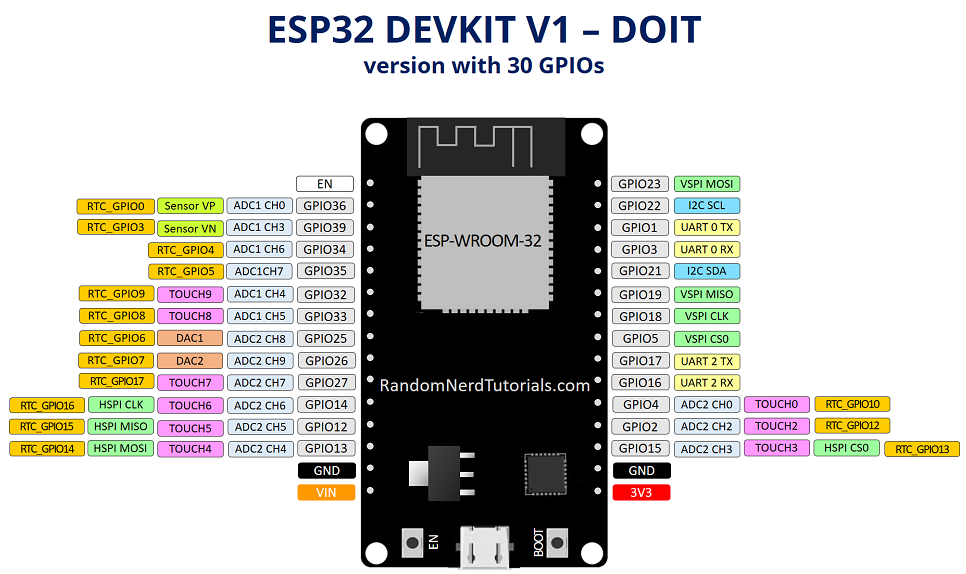
\includegraphics[scale = 0.6]{Hinhve/ESP32-DOIT-DEVKIT-V1.png}
    \centering
    \caption{Sơ đồ chân của module ESP32-WROOM-32 và chức năng từng chân}
\end{figure}

\section{Module điều khiển động cơ L298}
\label{section:3.5}

L298N là trình điều khiển động cơ H-Bridge kép cho phép điều khiển tốc độ và hướng của hai động cơ DC cùng một lúc. Module có thể điều khiển động cơ DC có điện áp trong khoảng từ 5 đến 35V, với dòng điện cực đại lên đến 2A.

\begin{figure}[H]
    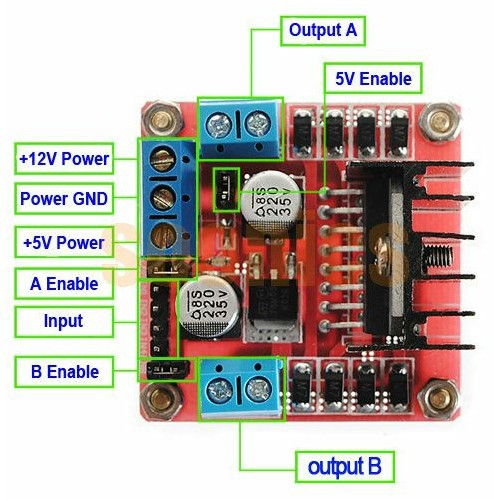
\includegraphics[scale = 0.6]{Hinhve/L298.jpg}
    \centering
    \caption{Sơ đồ chân của module L298}
\end{figure}

Cách thức hoạt động: Module này có hai nhóm chân cho động cơ A và B, và một chân ở giữa cho chân Ground, VCC cho động cơ và chân 5V có thể là đầu vào hoặc đầu ra. Điều này phụ thuộc vào điện áp được sử dụng tại động cơ VCC. Module L298 có bộ điều chỉnh 5V trên board được bật hoặc tắt bằng cách sử dụng dây nối. Nếu điện áp cung cấp động cơ lên đến 12V, thì có thể kích hoạt bộ điều chỉnh 5V và chân 5V có thể được sử dụng làm đầu ra, ví dụ để cấp nguồn cho board Arduino. Nhưng nếu điện áp động cơ lớn hơn 12V, cần phải ngắt kết nối dây vì những điện áp đó sẽ làm hỏng cho bộ điều chỉnh 5V trên board. Trong trường hợp này, chân 5V sẽ được sử dụng làm đầu vào vì mình cần kết nối nó với nguồn điện 5V để IC hoạt động bình thường.

Cách thức đấu dây trên mô hình thực tế được mô tả như hình dưới:

\begin{figure}[H]
    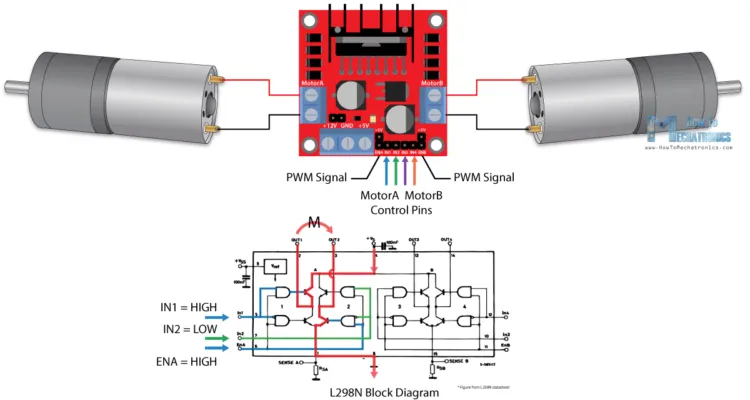
\includegraphics[scale = 0.6]{Hinhve/L298N-Block-Diagram.png}
    \centering
    \caption{Cách ghép nối L298 với động cơ}
\end{figure}

\section{Module LM2596}
\label{section:3.5}

Module LM2596 là mạch giảm áp DC nhỏ gọn có khả năng giảm áp từ 30V xuống 1.5V mà vẫn đạt hiệu suất cao (92\%). Thích hợp cho các ứng dụng chia nguồn, hạ áp, cấp cho các thiết bị như xe mô hình, motor, robot.

Thông số kỹ thuật:
\begin{itemize}
    \item Điện áp đầu vào: từ 3V đến 30V.
    \item Điện áp đầu ra: Điều chỉnh được trong khoảng 1.5V đến 30V.
    \item Dòng đáp ứng tối đa là 3V.
    \item Hiệu suất: 92\%.
    \item Công suất: 15W.
    \item Kích thước: 45 (dài) x 20 (rộng) x 14 (cao) mm
\end{itemize}

\begin{figure}[H]
    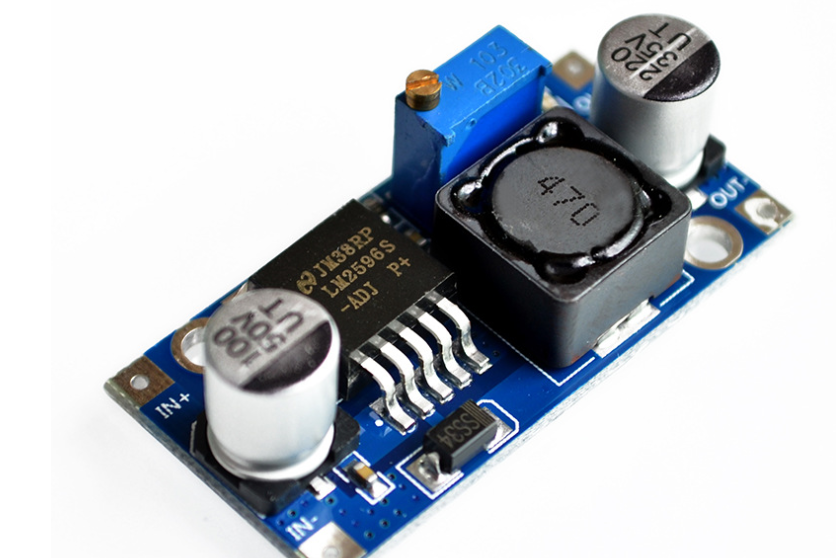
\includegraphics[scale = 0.6]{Hinhve/LM2596.png}
    \centering
    \caption{Sơ đồ chân của module LM2596}
\end{figure}

Cách sử dụng: Module có 2 đầu vào IN, OUT và một biến trở để chỉnh áp đầu ra. Khi cấp điện cho đầu vào (IN) thì người dùng vặn biến trở và dùng VOM để đo mức áp ở đầu ra (OUT) để đạt mức điện áp mong muốn. Điện áp đầu vào từ 4-35V, điện áp ra từ 1,25 - 30V, dòng tối ra 3A, có thể cấp nguồn sử dụng tốt cho raspberry và module sim...

\section{Cảm biến siêu âm HC-SR04}
\label{section:3.6}

HC-SR04 là cảm biến siêu âm chủ yếu được sử dụng để xác định khoảng cách của đối tượng mục tiêu. Nó đo khoảng cách chính xác bằng công nghệ không tiếp xúc, tức là không có tiếp xúc vật lý giữa cảm biến và vật thể.

\begin{figure}[H]
    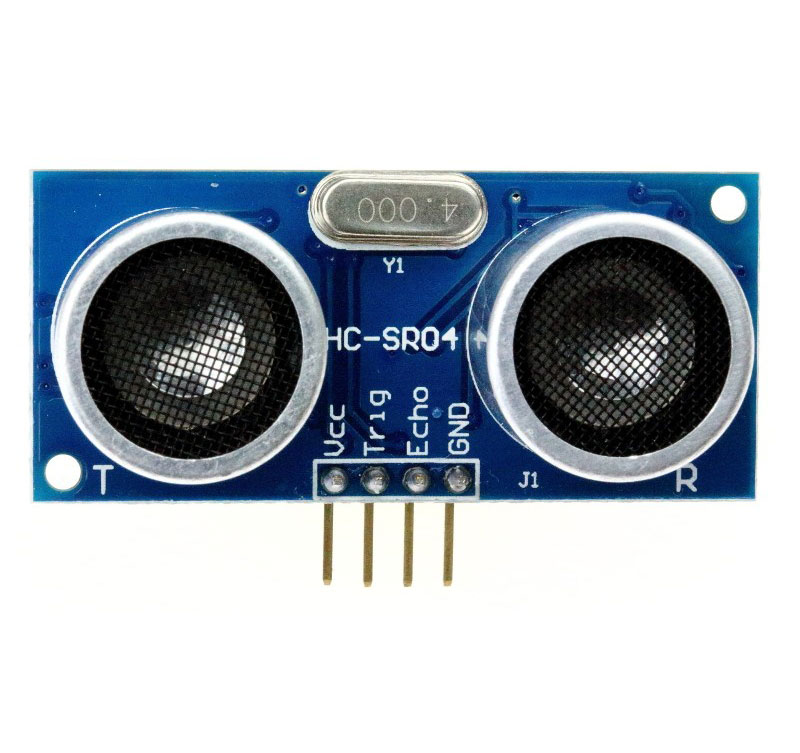
\includegraphics[scale = 0.5]{Hinhve/hcsr04.jpg}
    \centering
    \caption{Sơ đồ chân của Cảm biến siêu âm HC-SR04}
\end{figure}

Bộ phát và bộ thu là hai bộ phận chính của cảm biến, bộ phát chuyển đổi tín hiệu điện thành sóng siêu âm, còn bộ thu chuyển đổi tín hiệu siêu âm đó trở lại thành tín hiệu điện. Các sóng siêu âm này là các tín hiệu âm thanh có thể được đo và hiển thị ở đầu nhận.

\noindent\begin{minipage}{\linewidth}
\centering
\begin{tabular}{|p{2cm}|p{3cm}|p{10cm}|} 
\hline
\rowcolor[rgb]{1,0.808,0.576} \textbf{Số chân} & \textbf{Tên chân} & \textbf{Mô tả} \\ 
\hline
1 & Vcc & Chân Vcc cấp nguồn cho cảm biến, thường là +5V \\ 
\hline
2 & Trigger & Chân trigger là chân đầu vào. Chân này phải được giữ ở mức cao trong 10us để khởi tạo phép đo bằng cách gửi sóng siêu âm. \\ 
\hline
3 & Echo & Chân echo là chân đầu ra. Chân này tăng cao trong một khoảng thời gian bằng với thời gian để sóng siêu âm quay trở lại cảm biến. \\ 
\hline
4 & Ground & Chân nối đất. \\
\hline
\end{tabular}
\captionof{table}{Sơ đồ chân HC-SR04 và chức năng}
\end{minipage}

Tính năng, thông số kỹ thuật cảm biến HC-SR04
\begin{itemize}
    \item Điện áp hoạt động: +5V.
    \item Khoảng cách đo lý thuyết: 2cm đến 450cm.
    \item Khoảng cách đo thực tế: 2cm đến 80cm.
    \item Độ chính xác: 3mm.
    \item Góc đo được bao phủ: < 15 độ.
    \item Dòng điện hoạt động: < 15mA.
    \item Tần số hoạt động: 40Hz.
\end{itemize}

\end{document}